% Условная компиляция для самостоятельной работы
\ifdefined\mainfile
    % Если это часть основного файла, не добавляем начало и конец документа
\else
    \documentclass[12pt, a4paper]{report}
    \usepackage{/Users/vladbelousov/Desktop/Semestr_4-FP-NSU/Настройка/library}
    \usepackage[utf8]{inputenc} % Подключение поддержки UTF-8
    \begin{document}
\fi

%%-------------------------------%%

\chapter{Теория устойчивости}

\section{Основные определения}

Маятник длинной \( l \)  в поле тяжести \( g  \), отклоненный от положения устойчивости на угол \( \varphi \):

\[ \begin{cases}
    l \ddot{\varphi } + g \sin  \varphi = 0 \\
    \varphi (0 ) = 0  \kern +2cm  \Rightarrow \varphi ^{* }  (t ) = 0\\ 
    \dot{ \varphi } (0 ) = 0 
\end{cases} \] 
Частный случай: 

\[ \begin{cases}
l \ddot{\varphi } + g \sin  \varphi = 0 \\ 
\varphi( 0 ) = \pi \kern+2cm \Rightarrow \varphi^{** } (t ) = \pi \\ 
\dot{\varphi } (0 )  = 0  
\end{cases} \] 

\[ \begin{cases}
l \ddot{\varphi } + g \sin  \varphi = 0 \\ 
\varphi (0 )= \varphi_0 \kern+2cm \Rightarrow \varphi(t, \varphi_0 , \omega_0 ) \text{ - решение} \\
\dot{ \varphi } (0 ) = \omega_0 
\end{cases} \] 



\[ \begin{cases}
l \ddot{\varphi } + g \sin  \varphi = 0 \\ 
\varphi(0 ) = \pi + \varphi_0 \kern+2cm \Rightarrow \varphi(t , \pi + \varphi_0 , \omega_0 ) \text{ - решение} \\
\dot{ \varphi } (0 ) = \omega_0 
\end{cases} \] 

Непрерывная зависимость от начальных данных  - есть на конечном  отрезке времени. 

Устойчивость - непрерывная зависимость от начальных данных при \( t  \)  до \( 0  \)  до \( + \infty  \) 

\[
\displaystyle  \frac{d}{ dt } \vec{y }  = \vec{f }  (t, \vec{y }  ) 
\] 

\[ \vec{y }  =\begin{pmatrix}
y_1\\
\vdots\\
y_n
\end{pmatrix}, \text{ } \vec{f }  = \begin{pmatrix}
f_1     \\
\vdots\\
f_n
\end{pmatrix} , \text{ }  f_j : \mathbb{D} \to  \mathbb{R} ,\text{ }  \mathbb{D} \subset \mathbb{R}^{n+1 }  \text{ - непустое открытое} \] 

\[ \forall  j = 1, \ldots, n , \text{ }  f_j \in  C(\mathbb{D} ) , \text{ }  \forall  i,j = 1, \ldots, n \text{ }  \exists \frac{\partial  f_i }{\partial  y_j } \in  C(\mathbb{D})  \] 

\[ \begin{aligned}
    \begin{cases}
        \displaystyle \frac{d}{dt }  \vec{y } = \vec{f }  (t, \vec{y } ) \\
        \vec{y }  (t_0 ) = \vec{y }  ^{* }  _0
    \end{cases}
    \Rightarrow \text{ решение } \vec{y } ^* (t)  
\end{aligned} \] 

\[ \begin{aligned}
    \begin{cases}
        \displaystyle  \frac{d}{dt }  \vec{y }  = \vec{f }  (t, \vec{y}  )\\ 
        \vec{y } (t_0) = \vec{y }  _0
    \end{cases}
    \Rightarrow \text{ решение } \vec{y } (t)
\end{aligned} \]

\begin{definition}
    Решение \( \vec{y } ^*(t )   \) называется устойчивым по Ляпунову, если: 

    1) \( \vec{y } ^* (t ) \) определена от \( t_0  \) до \( +\infty  \)!

    \begin{center}
        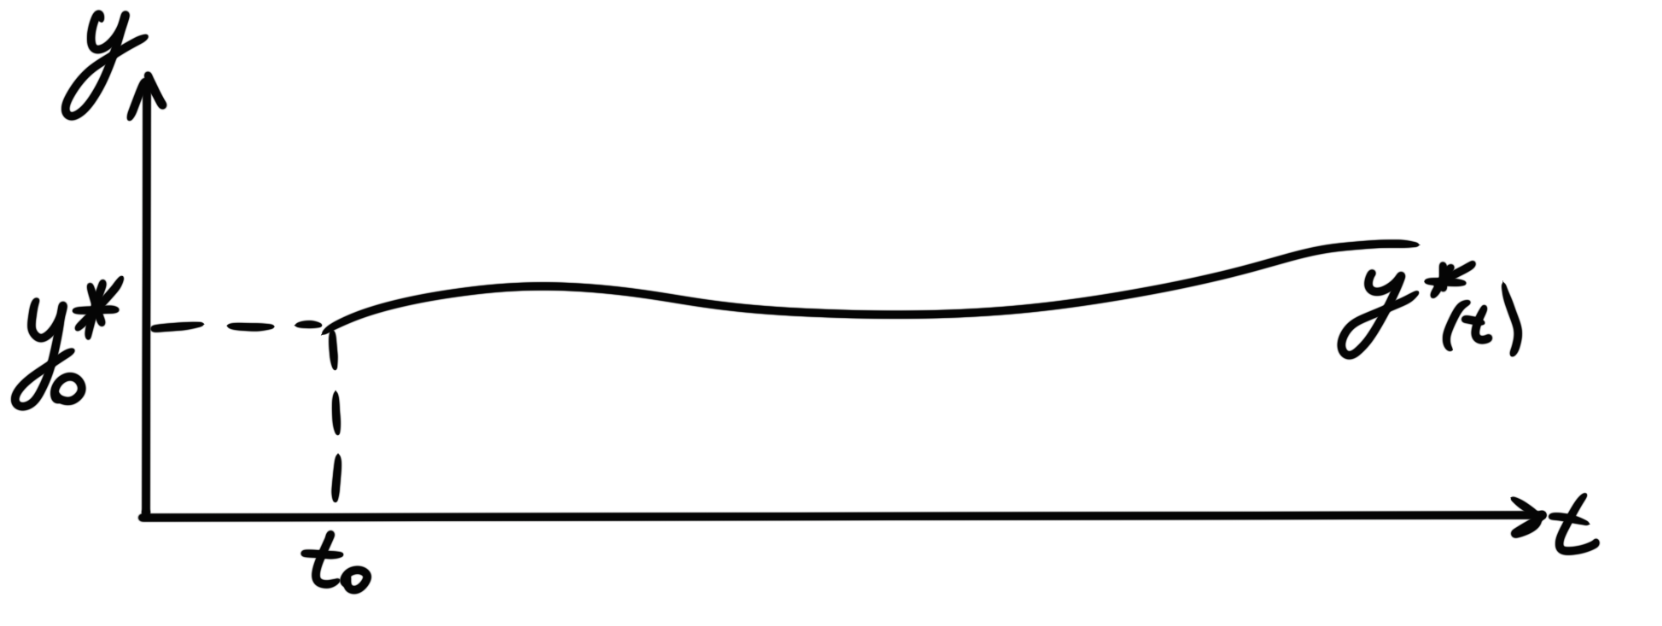
\includegraphics[width=0.6\textwidth]{/Users/vladbelousov/Desktop/Semestr_4-FP-NSU/ДфУ/Лекции_по_дням/image/31.png}
    \end{center}

    2) \( \exists \Delta > 0 \text{ }  \forall  \vec{y} _0 :   \left\lVert \vec{y } _ 0 - \vec{y } _0 ^*  \right\rVert< \Delta \Rightarrow \vec{y } (t )  \) тоже определенно от \( t_0  \) до \( +\infty  \)!

    \begin{center}
        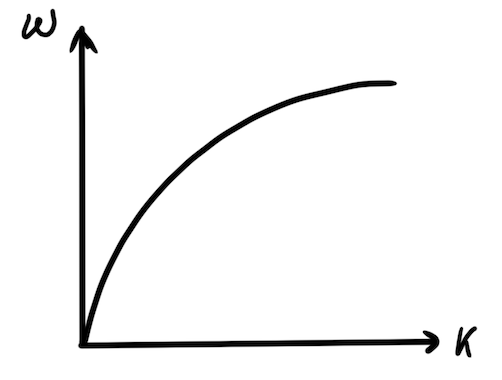
\includegraphics[width=0.6\textwidth]{/Users/vladbelousov/Desktop/Semestr_4-FP-NSU/ДфУ/Лекции_по_дням/image/32.png}
    \end{center}

    3) \( \forall  \varepsilon > 0 \text{ }  \exists  \delta > 0 \text{ }  \forall  \vec{y } _ 0 : \left\lVert  \vec{y } _0 - \vec{y }  ^ * _0  \right\rVert < \delta \Rightarrow \left\lVert  \vec{y }  (t ) - \vec{y }  ^*    (t ) \right\rVert < \varepsilon \text{ }  \forall  t \ge t_0 \) 

    \begin{center}
        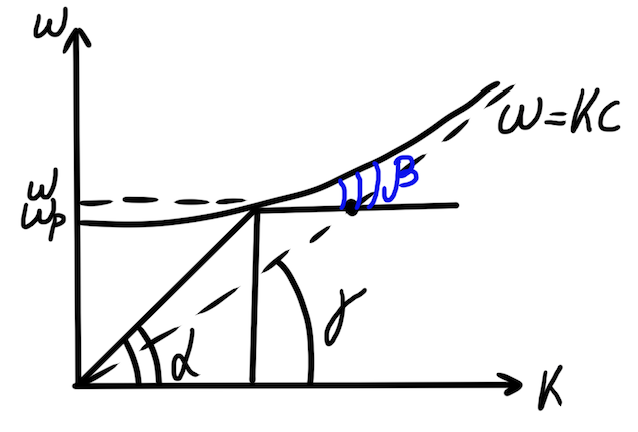
\includegraphics[width=0.6\textwidth]{/Users/vladbelousov/Desktop/Semestr_4-FP-NSU/ДфУ/Лекции_по_дням/image/33.png}
    \end{center}
\end{definition}

№1: Является ли устойчивое по Ляпунову решение задачи Коши: 

\[ \begin{cases}
y ' = 1 \\ 
y(0) = 0
\end{cases} \] 
\[ t_0 = 0, \text{ }  y^{* }  _0 = 0 , \text{ }  y^* (t )  = t \] 

1) \( y^* (t ) =t   \) определено от \( 0 \)  до \( + \infty  \)  (+)

\begin{center}
    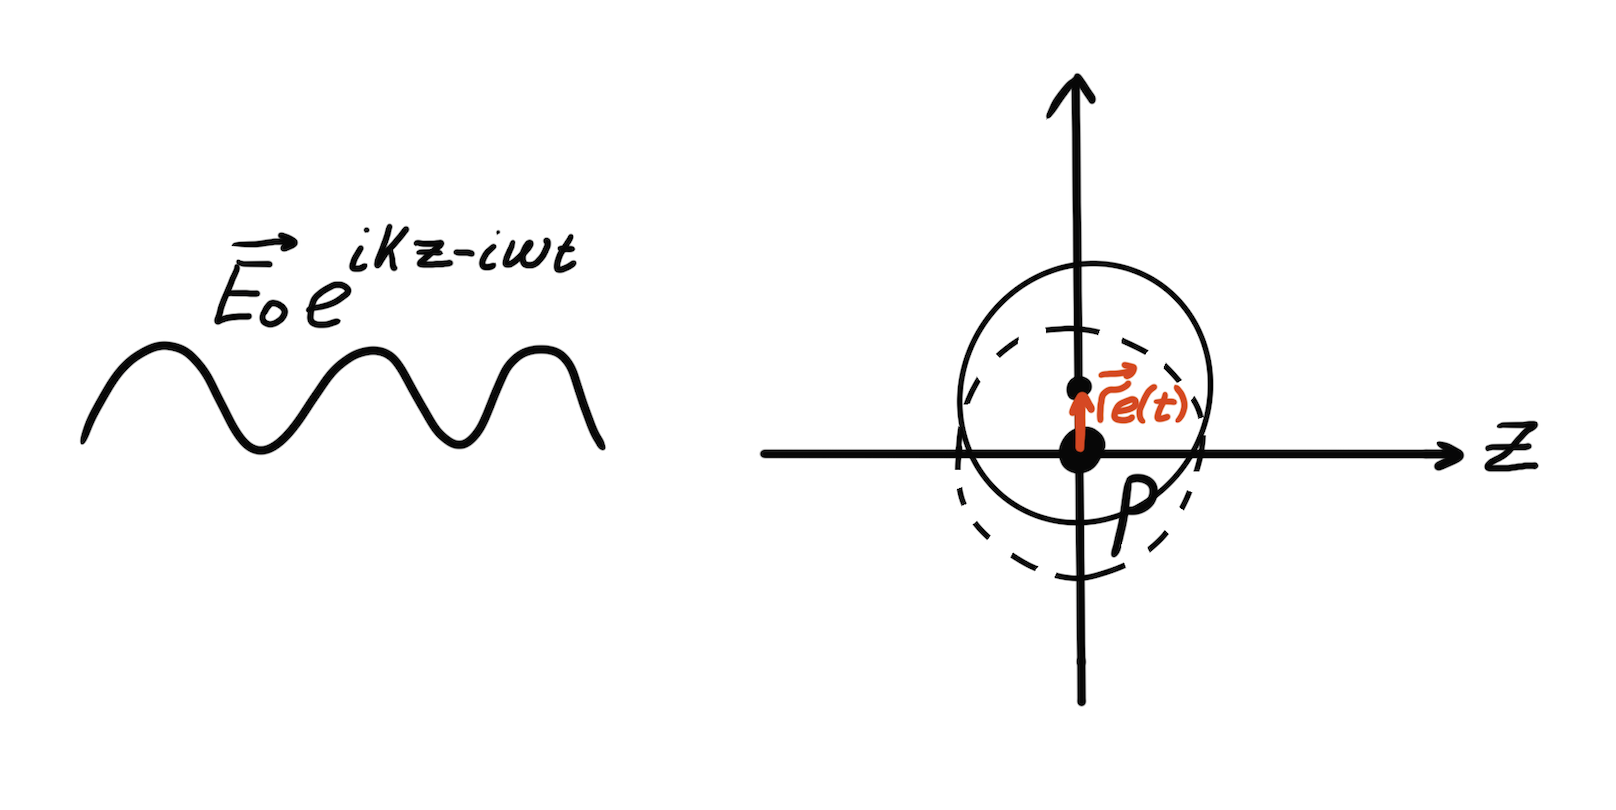
\includegraphics[width=0.4\textwidth]{/Users/vladbelousov/Desktop/Semestr_4-FP-NSU/ДфУ/Лекции_по_дням/image/34.png}
\end{center}

2) \( \begin{aligned}
    \begin{cases}
        y' = 1 \\ 
        y(0 )= 0 
    \end{cases}
    \Rightarrow y(t ) = t+ y_0
\end{aligned} \) (+)

\begin{center}
    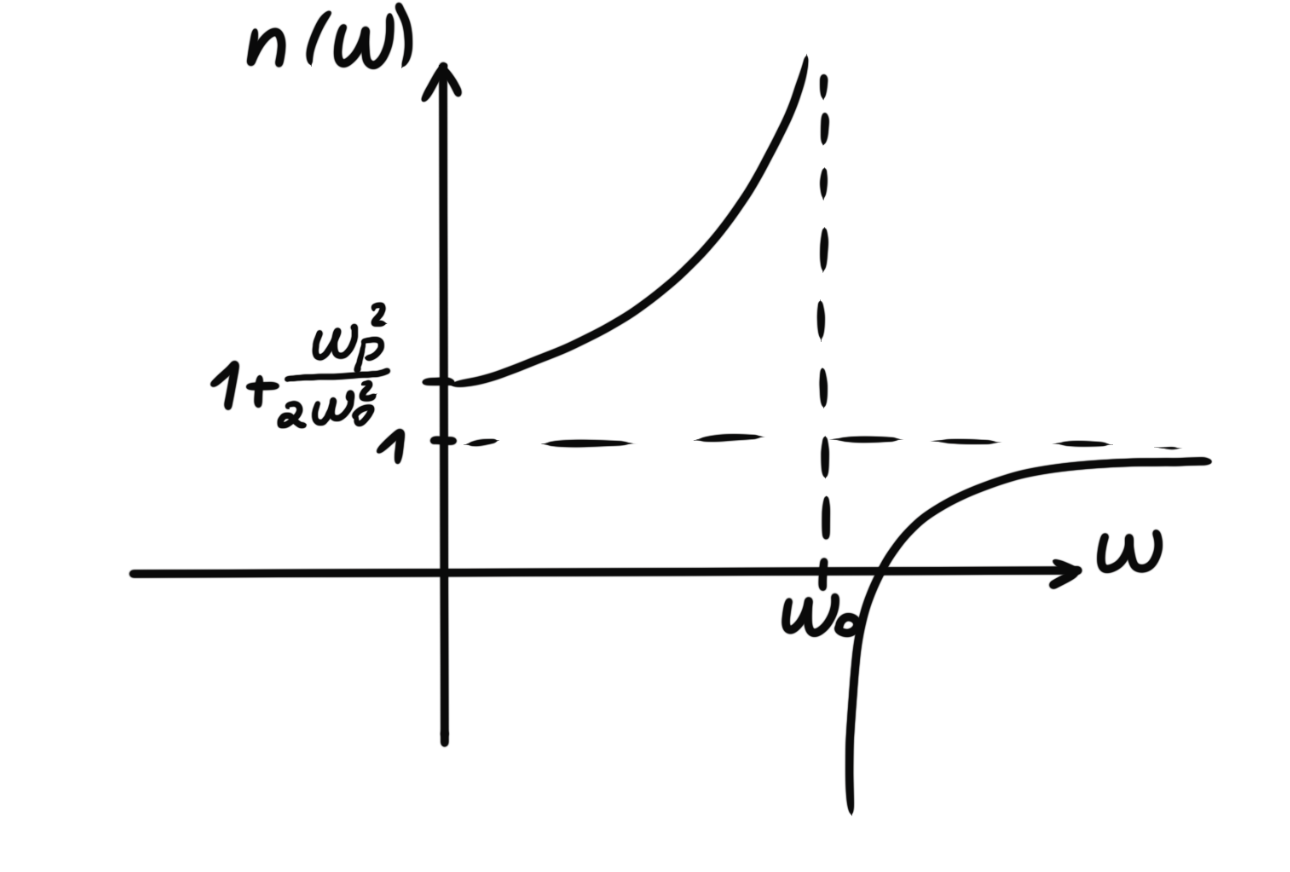
\includegraphics[width=0.4\textwidth]{/Users/vladbelousov/Desktop/Semestr_4-FP-NSU/ДфУ/Лекции_по_дням/image/35.png}
\end{center}

3) Надо показать: 

\[ \forall  \varepsilon > 0 \text{ }  \exists  \delta > 0 : \forall  y_0 : \left\lvert y_0  \right\rvert < \delta \Rightarrow\underbrace{ \left\lvert  y(t) - y^* (t )  \right\rvert}_{|y_0|} < \varepsilon \text{ } \forall  t \ge 0 \] 
\[ \delta = \varepsilon \Rightarrow \left\lvert y(t ) - y^ * (t )  \right\rvert = \left\lvert y_0 \right\rvert \] 

\begin{center}
    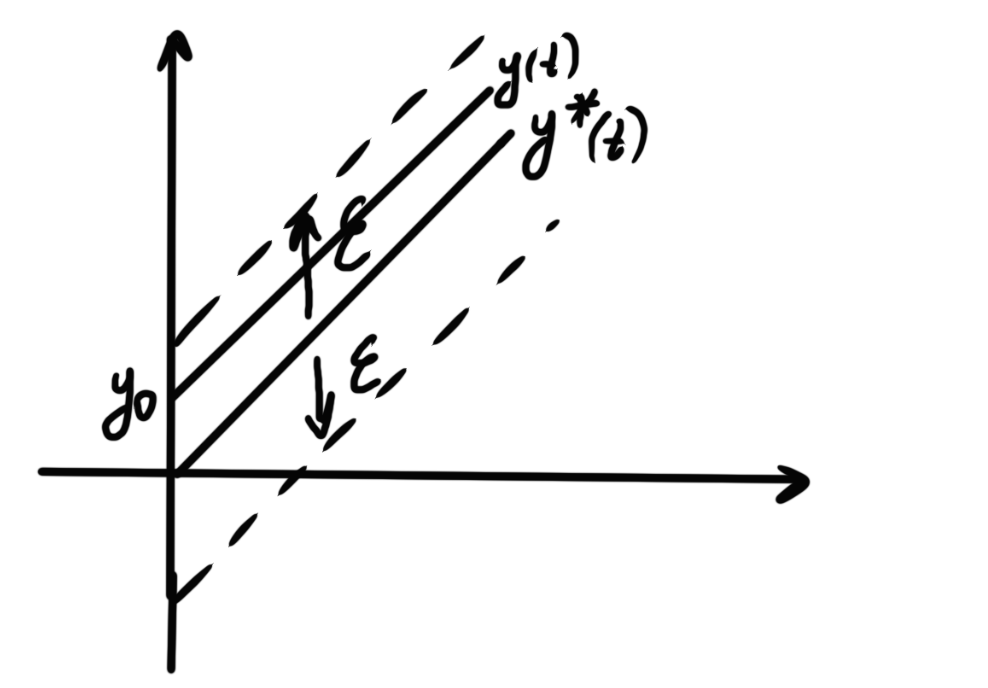
\includegraphics[width=0.4\textwidth]{/Users/vladbelousov/Desktop/Semestr_4-FP-NSU/ДфУ/Лекции_по_дням/image/36.png}
\end{center}

Ответ: \( y^* (t ) = t  \)  устойчиво по Ляпунову

\begin{definition}
    Решение \( \vec{y } ^* (t )  \) называется асимптотическим устойчивым, если: 

    1) \( \vec{y } ^* (t )  \) устойчиво по Ляпунову 

    2) \( \exists  \rho > 0 \text{ }  \forall  \vec{y } _0 : \left\lVert \vec{y } _ 0 - \vec{y }  ^* _0  \right\rVert < \rho \displaystyle \Rightarrow \lim_{t     \to \infty} \left\lVert \vec{y } (t ) - \vec{y}  ^* (t ) \right\rVert = 0  \) 

    \begin{center}
        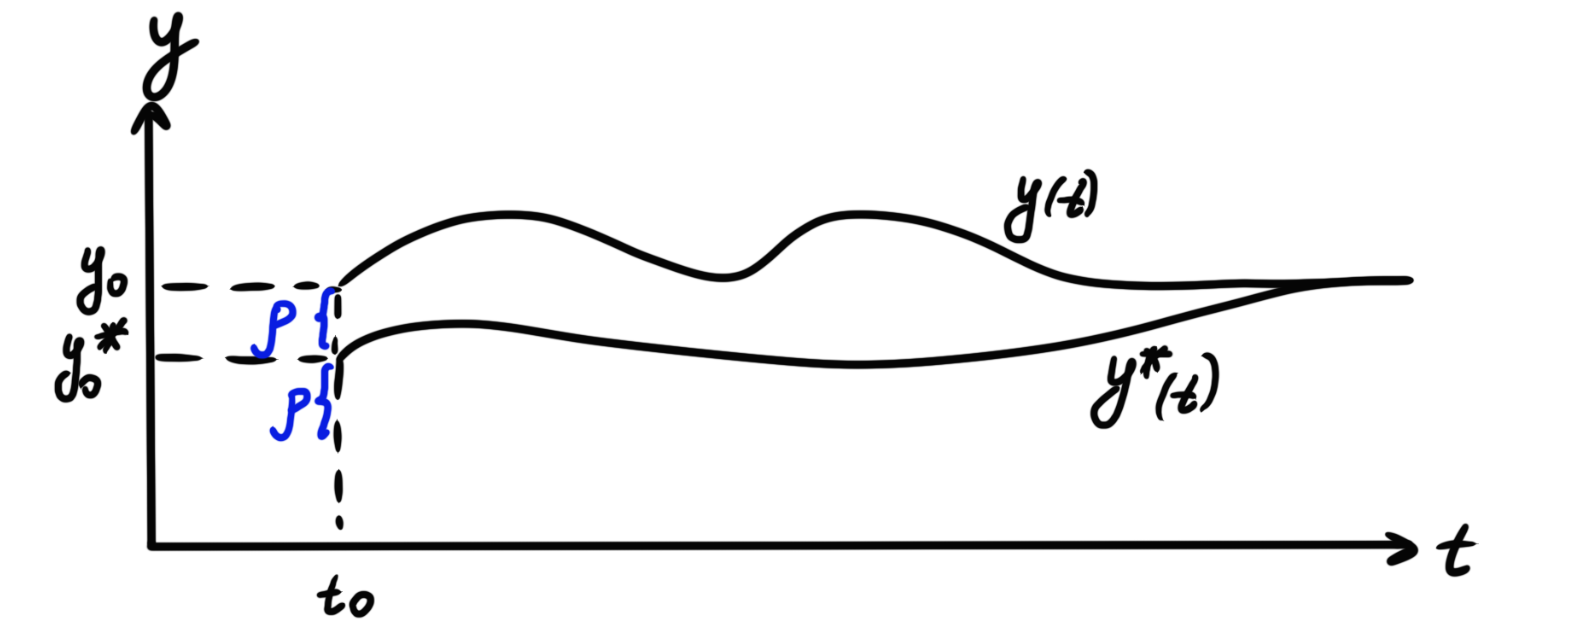
\includegraphics[width=0.6\textwidth]{/Users/vladbelousov/Desktop/Semestr_4-FP-NSU/ДфУ/Лекции_по_дням/image/37.png}
    \end{center}
\end{definition}

№2: Является ли устойчивое по Ляпунову асимптотическим устойчивым решение задачи Коши: 

\[ \begin{cases}
y ' = - y \\ 
y(0 )=  0
\end{cases} \] 
\[ t_0 = 0 , \text{ }  y_0 ^{* }  = 0  , \text{ }  y^{* }  (t ) = 0 \] 

\begin{center}
    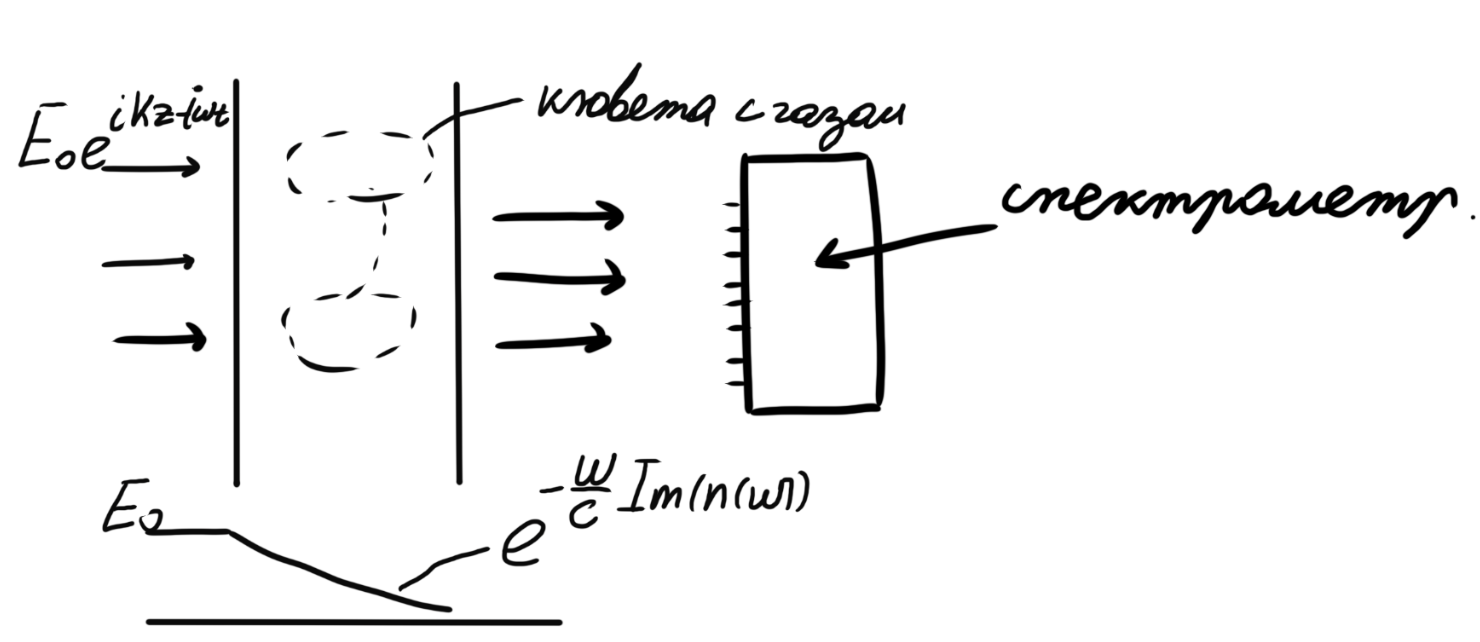
\includegraphics[width=0.4\textwidth]{/Users/vladbelousov/Desktop/Semestr_4-FP-NSU/ДфУ/Лекции_по_дням/image/38.png}
\end{center}

1) \( y^{* } (t ) = 0  \) определено на от \(  0 \)  до \( + \infty  \) (+)

2) \( \begin{aligned}
    \begin{cases}
        y ' = - y \\ 
        y(0 ) = y_0
    \end{cases}
    \Rightarrow y(t ) = e^{ - t } y_0 \text{ - определено на от } 0 \text{ до  }  + \infty  
\end{aligned} \) 

\begin{center}
    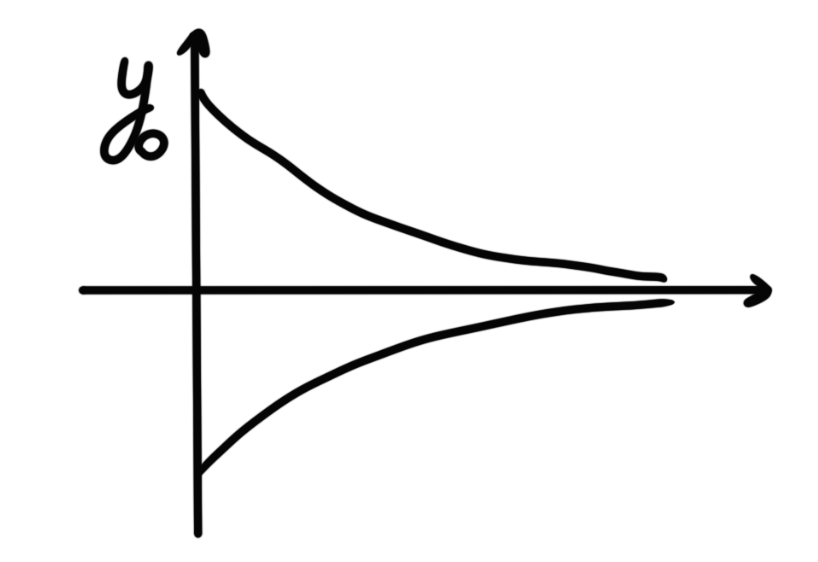
\includegraphics[width=0.4\textwidth]{/Users/vladbelousov/Desktop/Semestr_4-FP-NSU/ДфУ/Лекции_по_дням/image/39.png}
\end{center}

3) \( \forall  \varepsilon > 0 \text{ }  \exists  \delta > 0 \text{ }  \forall  y_0 : \left\lvert y_0  \right\rvert< \delta \Rightarrow \underbrace{\left\lvert y (t) \right\rvert}_{\left\lvert y_0 e^{ - t}  \right\rvert} < \varepsilon \text{ }  \forall  t \ge t_0 \) 

Возьмем \( \delta = \varepsilon  \) 

Если \( \left\lvert y_0      \right\rvert < \delta = \varepsilon \Rightarrow \left\lvert y(t ) \right\rvert = \left\lvert y_0 e^{ - t }  \right\rvert = \left\lvert y_0  \right\rvert e^{ -t } < \varepsilon  \Rightarrow \) нулевое решение \( y^* (t )   = 0\) устойчиво по Ляпунову

4) \( \displaystyle  \lim_{t  \to \infty} \left\lvert y(t) - y^* (t )  \right\rvert = \lim_{t  \to \infty}  \left\lvert y_0 e^{- t }  \right\rvert = 0\) 

\( \rho \) - любое \( \Rightarrow y^* (t ) =0\)   асимптотическим устойчиво. 

\begin{definition}
    Решение \( \vec{y } ^* (t )  \) называется неустойчивым, если оно не является устойчивым по Ляпунову, то есть если не выполняется хотя бы один пункт в определении устойчивости по Ляпунову.
\end{definition}

Не выполняется пункт 1: \( y^* (t ) \) не определено от \( 0 \) до \( + \infty  \) 

Не выполняется пункт 2: 

\( \forall  \Delta > 0 \text{ }  \exists  \vec{y } _0 : \left\lVert \vec{y}  _0 - \vec{y } ^* _0  \right\rVert < \Delta  \), \( \vec{y } (t ) \) не определено от \( t_0 \) до \( + \infty  \) 

Не выполняется пункт 3: 

\( \exists \varepsilon > 0 \text{ }  \forall  \delta > 0 \text{ }  \exists  \vec{y } _0 : \left\lVert  \vec{y }  _0 - \vec{y } _ 0 ^*  \right\rVert < \delta \Rightarrow   \exists  \hat{t }  \ge t_0 : \left\lVert \vec{y } (\hat{ t } )- \vec{y } ^*    (\hat{ t } )  \right\rVert \ge \varepsilon  \) 

№3: 

\[\begin{aligned}
    \begin{cases}
        y ' = 1 + y ^2 \\ 
        y(0 ) = 0
    \end{cases} 
    \Rightarrow y^* (t ) = \mathrm{tg }  (t ) 
\end{aligned}\] 

\begin{center}
    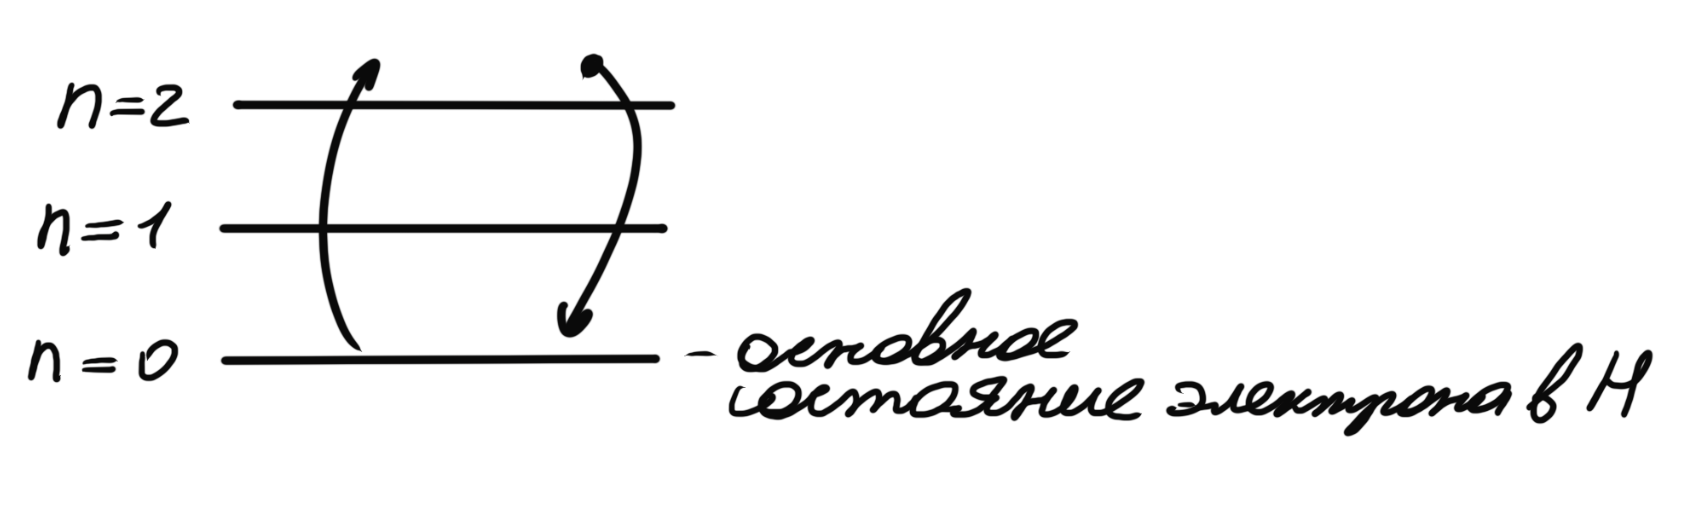
\includegraphics[width=0.3\textwidth]{/Users/vladbelousov/Desktop/Semestr_4-FP-NSU/ДфУ/Лекции_по_дням/image/40.png}
\end{center}

Не выполняется первый пункт \( \Rightarrow y^*(t ) = \mathrm{tg } (t ) \)  - неустойчиво. 

№4: 

\[ \begin{aligned}
    \begin{cases}
        y ' = y ^2 \\ 
        y(0 ) = 0
    \end{cases}
    \Rightarrow y^* (t ) = 0
\end{aligned} \] 

\begin{center}
    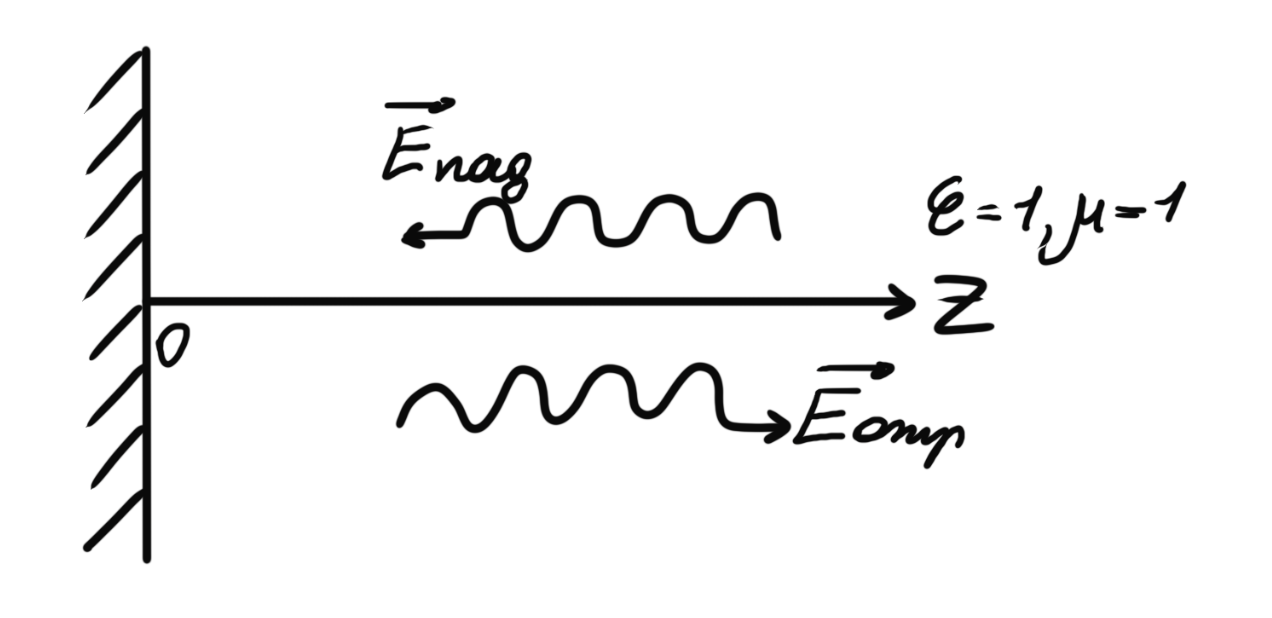
\includegraphics[width=0.4\textwidth]{/Users/vladbelousov/Desktop/Semestr_4-FP-NSU/ДфУ/Лекции_по_дням/image/41.png}
\end{center}

1) (+) \\



2) \( \begin{aligned}
\begin{cases}
    y' = y ^2 \\ 
    y(0 ) = y_0
\end{cases}
\Rightarrow y(t ) = \frac{1}{\displaystyle  \frac{1}{y_0 } -t  } 
\end{aligned} \) 

\[ y(t ) \text{ при }  y_0> 0 \text{ не определено от } 0 \text{ до }  + \infty   \Rightarrow 2) \text{ не выполняется}\Rightarrow y^{* } (t )= 0 \text{ - неустойчиво}  \] 

№5: 

\[ \begin{aligned}
\begin{cases}
y ' = y \\ 
y(0 ) = 0 
\end{cases}
\Rightarrow y^* (t ) = 0
\end{aligned} \] 

1) \( y^*  (t ) = 0\)  определено от \( 0 \) до \( + \infty  \)  (+)

2) \[ \begin{aligned}
\begin{cases}
y ' = y \\ 
y(0 ) = y_0 
\end{cases}
\Rightarrow y(t ) = y_0 e^{t } 
\end{aligned} \]

\begin{center}
    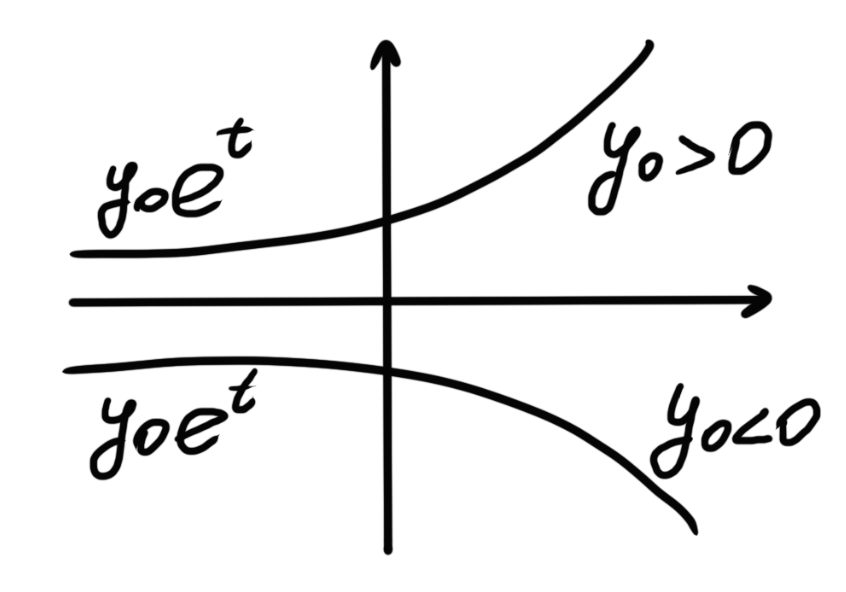
\includegraphics[width=0.4\textwidth]{/Users/vladbelousov/Desktop/Semestr_4-FP-NSU/ДфУ/Лекции_по_дням/image/42.png}
\end{center}

\[ y(t) \text{ определено от } 0 \text{ до }  + \infty  \quad  (+)  \] 

3) 

\begin{center}
    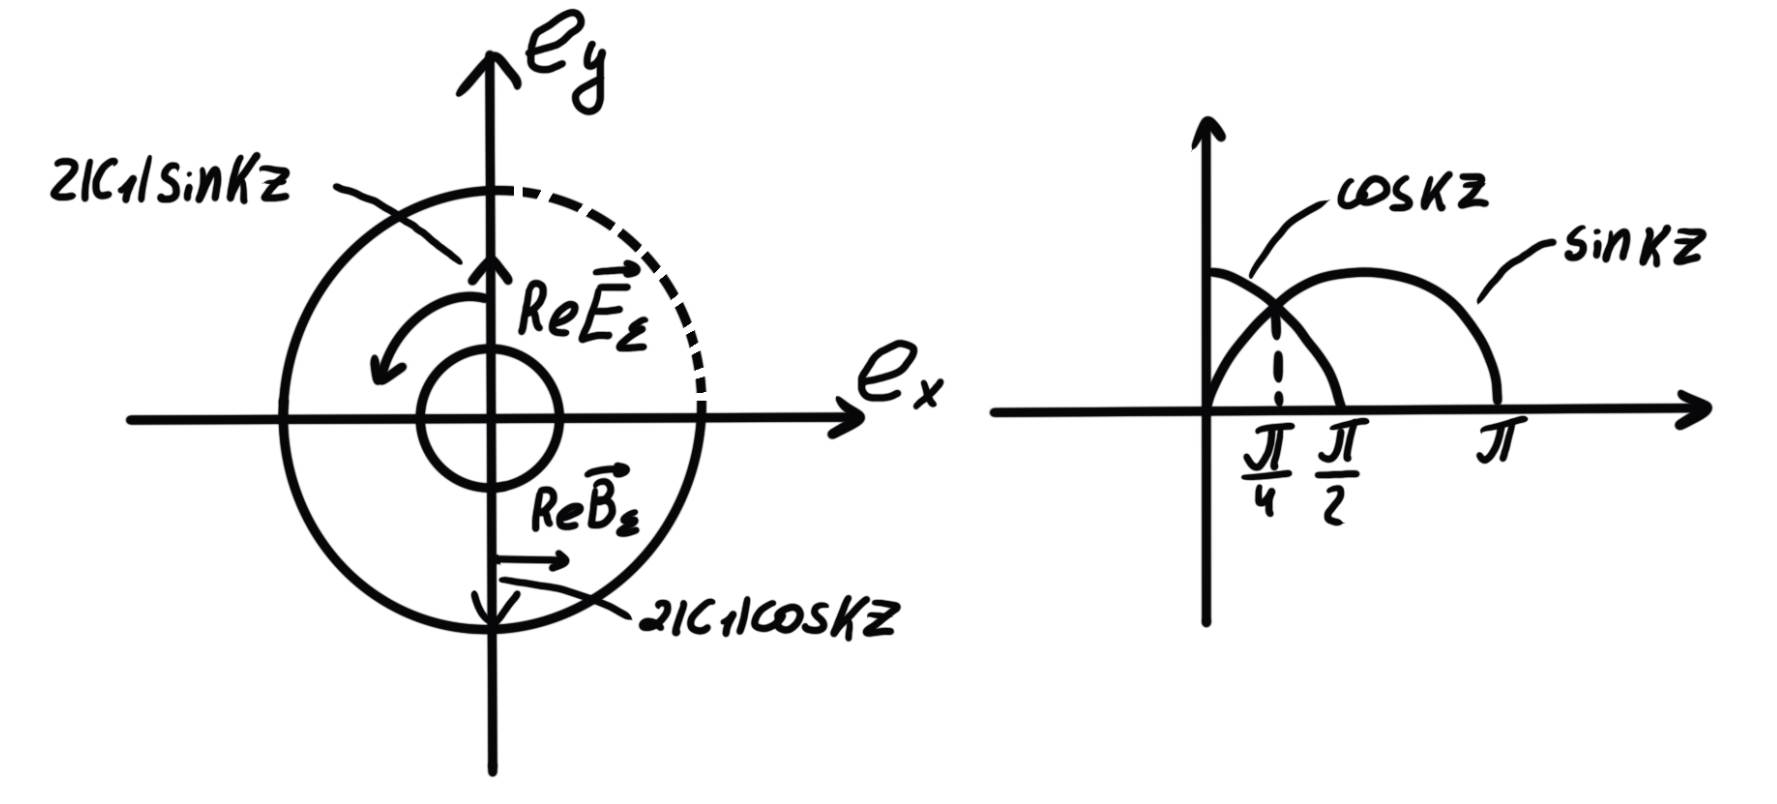
\includegraphics[width=0.4\textwidth]{/Users/vladbelousov/Desktop/Semestr_4-FP-NSU/ДфУ/Лекции_по_дням/image/43.png}
\end{center}

\[ \exists  \varepsilon = 10 \text{ }  \forall  \delta > 0 : \exists  y_0= \frac{\delta}{2 } : \left\lvert y_0  \right\rvert < \delta  \] 
\[ \exists \hat{ t }  : \left\lvert y(\hat{t }  ) \right\rvert \ge \varepsilon = 10 \] 
\[ \left\lvert y_0 e^{\hat{t } }  \right\rvert = \frac{\delta}{2 } e^{\hat{ t } } \] 

\[ \frac{\delta}{2 }  e^{\hat{ t } } \ge 10 \Rightarrow \hat{ t }  = \ln \left( \frac{20}{\delta}  \right)  \] 

Нулевое решение \( y^* (t ) = 0\)  неустойчиво.
%%-------------------------------%%

% Закрытие документа, если файл компилируется отдельно
\ifdefined\mainfile
    % Если это основной файл, не нужно заканчивать документ
\else
    \end{document}
\fi